% =====================================================================
% RESULTADOS E DISCUSSÃO
% Apresente os resultados (texto, tabelas, gráficos) e discuta-os à luz
% da fundamentação teórica. Este capítulo demonstra um gráfico com pgfplots.
% =====================================================================

Lorem ipsum dolor sit amet, consectetur adipiscing elit, sed do eiusmod tempor
incididunt ut labore et dolore magna aliqua. Os resultados são apresentados na
\autoref{fig:grafico} e discutidos a seguir.

%-------------------------------------------------------------
\section{Resultados}
\label{sec:resultados}
%-------------------------------------------------------------

% --- EXEMPLO DE GRÁFICO (pgfplots, autocontido) ----------------------
\begin{figure}[!htb]
  \caption{Exemplo de gráfico de barras gerado com pgfplots.}
  \label{fig:grafico}
  \centering
  % A fonte fica alinhada à margem esquerda DO GRÁFICO (não do texto).
  \elementocomfonte{%
  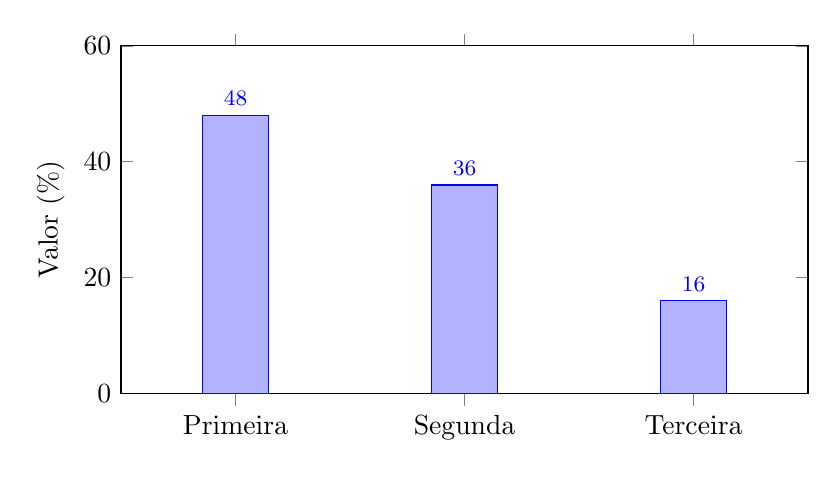
\begin{tikzpicture}
  \begin{axis}[
    ybar, width=0.85\textwidth, height=6cm,
    symbolic x coords={Primeira,Segunda,Terceira},
    xtick=data,
    ylabel={Valor (\%)},
    ymin=0, ymax=60,
    bar width=24pt,
    nodes near coords, nodes near coords style={font=\footnotesize},
    enlarge x limits=0.25,
  ]
  \addplot coordinates {(Primeira,48) (Segunda,36) (Terceira,16)};
  \end{axis}
  \end{tikzpicture}}%
  {Fonte: Elaborada pelo autor (\the\year{}).}
\end{figure}

Ut enim ad minim veniam, quis nostrud exercitation ullamco laboris nisi ut
aliquip ex ea commodo consequat~\parencite{exemplo-artigo}.

%-------------------------------------------------------------
\section{Discussão}
\label{sec:discussao}
%-------------------------------------------------------------

Duis aute irure dolor in reprehenderit in voluptate velit esse cillum dolore eu
fugiat nulla pariatur. Os achados são coerentes com \textcite{exemplo-livro} e
contrastam com parte da literatura, sugerindo que [interprete aqui os seus
resultados].
